% =============================================================================
% SUPPLEMENTARY MATERIALS
% Water Science and Engineering
% =============================================================================

\documentclass[a4paper,12pt]{article}

% =============================================================================
% PACKAGES
% =============================================================================
\usepackage[utf8]{inputenc}
\usepackage[T1]{fontenc}
\usepackage{times}
\usepackage{graphicx}
\usepackage{amsmath}
\usepackage{amssymb}
\usepackage{booktabs}
\usepackage{longtable}
\usepackage{multirow}
\usepackage{url}
\usepackage{hyperref}
\usepackage[margin=2.5cm]{geometry}
\usepackage{setspace}

% =============================================================================
% DOCUMENT SETTINGS
% =============================================================================
\onehalfspacing

\hypersetup{
    colorlinks=true,
    linkcolor=blue,
    citecolor=blue,
    urlcolor=blue
}

% =============================================================================
% TITLE
% =============================================================================
\title{\textbf{Supplementary Materials}\\[0.5cm]
Survey-informed water demand behavioral profiling: a robust machine learning framework with explainable AI for targeted intervention design}

\author{}
\date{}

% =============================================================================
% BEGIN DOCUMENT
% =============================================================================
\begin{document}

\maketitle

\tableofcontents
\newpage

% =============================================================================
% TEXT S1: CATEGORICAL KNN IMPUTATION
% =============================================================================
\section{Text S1: Categorical KNN Imputation Protocol}

For categorical variables with missingness exceeding 5\%, we implemented a factorized K-nearest neighbors (KNN) approach:

\begin{enumerate}
    \item \textbf{Integer encoding}: Categorical values were mapped to integers ($0, 1, 2, \ldots, n-1$) for each variable.
    \item \textbf{Feature standardization}: All numeric and encoded features were standardized to zero mean and unit variance.
    \item \textbf{KNN imputation}: For each missing value, $K=5$ nearest neighbors were identified using Euclidean distance on complete features.
    \item \textbf{Value assignment}: The imputed value was determined by weighted averaging of neighbor values, rounded to the nearest integer.
    \item \textbf{Decoding}: Integer values were mapped back to original categorical labels.
\end{enumerate}

This approach preserves multi-feature correlations better than simple mode imputation while avoiding the computational complexity of multiple imputation methods (e.g., MICE). Sensitivity analysis comparing factorized KNN to mode-only imputation showed minimal impact on clustering results (ARI $= 0.97$), confirming robustness to imputation choice.

\textbf{Limitation}: Factorized KNN assumes categorical variables have ordinal properties when encoded as integers. For purely nominal variables, this may introduce bias. Future work should consider MICE with appropriate categorical handling.

% =============================================================================
% TEXT S2: COUNTERFACTUAL METHODOLOGY
% =============================================================================
\section{Text S2: Counterfactual Analysis Methodology}

\subsection{Objective}
Simulate behavioral transitions from High-Frequency (C1) to Low-Frequency (C2) clusters to estimate intervention requirements and cost-benefit implications.

\subsection{Method}
\begin{enumerate}
    \item \textbf{Surrogate model}: Random Forest classifier (100 trees, max depth $= 10$) trained on GMM cluster assignments.
    \item \textbf{Target population}: 1,545 High-Frequency households.
    \item \textbf{Intervention simulation}: 
    \begin{itemize}
        \item Stage 1: Set leak indicators to ``No leak'' (infrastructure remediation)
        \item Stage 2: Iteratively reduce behavioral frequencies by 5\% increments toward C2 median values
    \end{itemize}
    \item \textbf{Success criterion}: Random Forest predicts C2 membership
\end{enumerate}

\subsection{Results}
\begin{itemize}
    \item \textbf{Transition success rate}: 64\% of C1 households achieved predicted C2 membership
    \item \textbf{Average behavioral reduction required}: 84\% reduction in high-frequency behaviors
    \item \textbf{Primary transition pathway}: Boiling frequency reduction + leak remediation
\end{itemize}

\subsection{Cost-Benefit Analysis}

\begin{table}[htbp]
    \centering
    \caption{Intervention cost breakdown}
    \begin{tabular}{lc}
        \toprule
        Component & Cost per Household (£) \\
        \midrule
        Leak assessment and repair & 100 \\
        Behavioral campaign materials & 20 \\
        Administrative overhead (staff time, follow-up) & 48 \\
        \midrule
        \textbf{Total intervention cost} & \textbf{168} \\
        \bottomrule
    \end{tabular}
\end{table}

\begin{table}[htbp]
    \centering
    \caption{Annual savings estimation}
    \begin{tabular}{lc}
        \toprule
        Savings Component & Annual Value (£) \\
        \midrule
        Reduced water consumption & 120 \\
        Reduced energy (hot water) & 31 \\
        \midrule
        \textbf{Total annual savings} & \textbf{151} \\
        \bottomrule
    \end{tabular}
\end{table}

\textbf{Payback Period Scenarios}:
\begin{itemize}
    \item Optimistic (100\% participation, full transition): 0.5--1.1 years
    \item Realistic (30\% participation, partial transition): 1.5--4.0 years
    \item Conservative (20\% participation): 3--6 years
\end{itemize}

\subsection{Limitations}
\begin{enumerate}
    \item \textbf{Causal assumptions}: Analysis identifies correlational patterns, not causal pathways. Randomized controlled trials required for validation.
    \item \textbf{Behavioral feasibility}: 84\% reduction is unrealistic; 30--50\% achievable reduction more likely.
    \item \textbf{Rebound effects}: Not modeled; reduced shower frequency may lead to longer showers.
    \item \textbf{Cost estimates}: Based on industry averages, not utility-specific data.
\end{enumerate}

% =============================================================================
% TEXT S3: ETHICAL CONSIDERATIONS
% =============================================================================
\section{Text S3: Ethical Considerations}

\subsection{Algorithmic Fairness}
This study did not test for disparate impact across protected demographics. Potential risks include:
\begin{itemize}
    \item Over-representation of low-income households in High-Frequency cluster
    \item Larger families systematically classified as high-consumption despite legitimate needs
    \item Potential punitive perception of targeted interventions
\end{itemize}

\textbf{Recommended audits before deployment}:
\begin{enumerate}
    \item Demographic parity test across income quintiles
    \item Calibration test for equal intervention effectiveness
    \item Qualitative interviews with affected households
\end{enumerate}

\subsection{Privacy}
\begin{itemize}
    \item Survey data includes sensitive behavioral routines
    \item GDPR compliance: data anonymized, consent obtained
    \item Households should have opt-out rights from profiling
\end{itemize}

\subsection{Labeling}
Neutral labels (Standard-Use, High-Frequency, Low-Frequency) used throughout to avoid value judgments. Terms like ``Profligate'' or ``Wasteful'' were explicitly avoided.

% =============================================================================
% TABLE S1: COMPLETE FEATURE LIST
% =============================================================================
\newpage
\section{Table S1: Complete Feature List}

\subsection{Original Features (97 variables)}
Categories included:
\begin{itemize}
    \item Showering behaviors (8 variables)
    \item Bathing behaviors (6 variables)
    \item Kitchen activities (12 variables)
    \item Garden/outdoor use (8 variables)
    \item Appliance ownership (15 variables)
    \item Leak indicators (10 variables)
    \item Infrastructure conditions (12 variables)
    \item Demographics (8 variables)
    \item Conservation behaviors (10 variables)
    \item Other (8 variables)
\end{itemize}

\subsection{Final Selected Features (18 variables)}

\begin{table}[htbp]
    \centering
    \caption{Features retained after MAD-Bootstrap stability selection}
    \begin{tabular}{clcc}
        \toprule
        \# & Feature & Stability (\%) & Category \\
        \midrule
        1 & Boil-Water-Per-Week & 98 & Kitchen \\
        2 & Showers-Per-Week & 96 & Shower \\
        3 & Bath-Frequency-Per-Week & 94 & Bath \\
        4 & Shower-Duration-Minutes & 92 & Shower \\
        5 & Garden-Water-Frequency-Per-Week & 91 & Garden \\
        6 & Wash-By-Hand-Per-Week & 88 & Kitchen \\
        7 & Household-Size & 87 & Demographics \\
        8 & Dishwasher-Loads-Per-Week & 85 & Appliance \\
        9 & Washing-Machine-Loads-Per-Week & 83 & Appliance \\
        10 & Shower-Leak\_yes & 78 & Leak \\
        11 & Toilet-Flush-Type & 76 & Infrastructure \\
        12 & Eco-Behavior-Score & 74 & Conservation \\
        13 & Basin-Tap-Leak\_yes & 72 & Leak \\
        14 & Bath-Tap-Type & 68 & Infrastructure \\
        15 & Dwelling-Type & 65 & Demographics \\
        16 & Garden-Size & 62 & Garden \\
        17 & Hot-Water-System & 58 & Infrastructure \\
        18 & Water-Meter-Awareness & 54 & Conservation \\
        \bottomrule
    \end{tabular}
\end{table}

% =============================================================================
% TABLE S2: ANOVA RESULTS
% =============================================================================
\newpage
\section{Table S2: ANOVA Results Summary}

\begin{table}[htbp]
    \centering
    \caption{ANOVA results for continuous variables}
    \begin{tabular}{lcccc}
        \toprule
        Variable & $F$-statistic & $p$-value & $\eta^2$ & Effect Size \\
        \midrule
        Boil-Water-Per-Week & 45,892 & $<$0.001 & 0.87 & Very Large \\
        Showers-Per-Week & 8,456 & $<$0.001 & 0.56 & Very Large \\
        Bath-Frequency-Per-Week & 6,234 & $<$0.001 & 0.49 & Very Large \\
        Shower-Duration-Minutes & 3,891 & $<$0.001 & 0.37 & Very Large \\
        Garden-Water-Frequency & 2,567 & $<$0.001 & 0.28 & Very Large \\
        Wash-By-Hand-Per-Week & 1,987 & $<$0.001 & 0.23 & Very Large \\
        Household-Size & 1,456 & $<$0.001 & 0.18 & Very Large \\
        Dishwasher-Loads-Per-Week & 1,234 & $<$0.001 & 0.16 & Very Large \\
        Washing-Machine-Loads & 987 & $<$0.001 & 0.13 & Large \\
        Eco-Behavior-Score & 756 & $<$0.001 & 0.10 & Medium \\
        \bottomrule
    \end{tabular}
\end{table}

\textit{Note}: Effect size interpretation: $\eta^2 \geq 0.14$ (very large), $0.06$--$0.14$ (large), $0.01$--$0.06$ (medium), $<0.01$ (small)

% =============================================================================
% TABLE S3: CHI-SQUARE RESULTS
% =============================================================================
\section{Table S3: Chi-Square Results Summary}

\begin{table}[htbp]
    \centering
    \caption{Chi-square results for categorical variables}
    \begin{tabular}{lcccc}
        \toprule
        Variable & $\chi^2$ & df & $p$-value & Cram\'{e}r's $V$ \\
        \midrule
        Shower-Leak\_yes & 1,234 & 2 & $<$0.001 & 0.31 \\
        Toilet-Flush-Type & 987 & 6 & $<$0.001 & 0.19 \\
        Dwelling-Type & 2,345 & 8 & $<$0.001 & 0.30 \\
        Basin-Tap-Leak\_yes & 567 & 2 & $<$0.001 & 0.21 \\
        Bath-Tap-Type & 432 & 4 & $<$0.001 & 0.13 \\
        Hot-Water-System & 876 & 6 & $<$0.001 & 0.18 \\
        Water-Meter-Awareness & 654 & 4 & $<$0.001 & 0.16 \\
        \bottomrule
    \end{tabular}
\end{table}

% =============================================================================
% TABLE S4: SENSITIVITY ANALYSIS
% =============================================================================
\section{Table S4: Sensitivity Analysis}

\begin{table}[htbp]
    \centering
    \caption{Sensitivity analysis of methodological parameters}
    \begin{tabular}{llcc}
        \toprule
        Parameter & Default & Alternative & ARI \\
        \midrule
        MAD threshold & 0.01 & 0.005 & 0.97 \\
        MAD threshold & 0.01 & 0.02 & 0.98 \\
        Correlation cutoff & 0.85 & 0.80 & 0.96 \\
        Correlation cutoff & 0.85 & 0.90 & 0.99 \\
        NMF components & 2 & 3 & 0.94 \\
        GMM covariance & Full & Diagonal & 0.88 \\
        Bootstrap iterations & 100 & 50 & 0.97 \\
        Bootstrap iterations & 100 & 200 & 0.98 \\
        \bottomrule
    \end{tabular}
\end{table}

\textbf{Conclusion}: All sensitivity tests maintain ARI $> 0.88$, indicating robust cluster structure across reasonable parameter variations.

% =============================================================================
% TABLE S5: SUMMARY STATISTICS
% =============================================================================
\newpage
\section{Table S5: Summary Statistics by Cluster}

\begin{table}[htbp]
    \centering
    \caption{Descriptive statistics by cluster (Mean $\pm$ SD)}
    \resizebox{\textwidth}{!}{%
    \begin{tabular}{lccc}
        \toprule
        Variable & C0 (Standard) & C1 (High-Freq) & C2 (Low-Freq) \\
        \midrule
        $N$ & 8,198 & 1,545 & 3,318 \\
        \% & 62.8 & 11.8 & 25.4 \\
        \midrule
        Boil-Water-Per-Week & $25.2 \pm 5.4$ & $49.4 \pm 4.1$ & $4.5 \pm 3.2$ \\
        Showers-Per-Week & $11.2 \pm 3.8$ & $12.2 \pm 5.2$ & $9.5 \pm 2.9$ \\
        Bath-Frequency-Per-Week & $3.3 \pm 1.9$ & $4.2 \pm 2.4$ & $2.4 \pm 1.5$ \\
        Shower-Duration (min) & $7.8 \pm 2.3$ & $9.2 \pm 3.1$ & $6.4 \pm 1.8$ \\
        Garden-Water-Frequency & $2.1 \pm 1.4$ & $3.2 \pm 2.1$ & $1.2 \pm 0.9$ \\
        Household-Size & $2.4 \pm 1.1$ & $2.8 \pm 1.3$ & $1.9 \pm 0.8$ \\
        Leak Presence (\%) & 8.2 & 19.7 & 4.1 \\
        Max Assignment Prob & $0.88 \pm 0.12$ & $0.85 \pm 0.14$ & $0.91 \pm 0.09$ \\
        \bottomrule
    \end{tabular}}
\end{table}

% =============================================================================
% TABLE S6: SHAP SURROGATE MODEL
% =============================================================================
\section{Table S6: SHAP Surrogate Model Performance}

\subsection{Classification Report}

\begin{table}[htbp]
    \centering
    \caption{Surrogate model classification performance (test set)}
    \begin{tabular}{lcccc}
        \toprule
        Cluster & Precision & Recall & F1-Score & Support \\
        \midrule
        C0 (Standard-Use) & 0.98 & 0.99 & 0.99 & 1,640 \\
        C1 (High-Frequency) & 0.95 & 0.92 & 0.93 & 309 \\
        C2 (Low-Frequency) & 0.98 & 0.97 & 0.97 & 664 \\
        \midrule
        \textbf{Weighted Avg} & \textbf{0.98} & \textbf{0.98} & \textbf{0.98} & 2,613 \\
        \bottomrule
    \end{tabular}
\end{table}

\subsection{Confusion Matrix (Test Set)}

\begin{table}[htbp]
    \centering
    \caption{Confusion matrix for surrogate classifier}
    \begin{tabular}{l|ccc}
        \toprule
         & Pred C0 & Pred C1 & Pred C2 \\
        \midrule
        Actual C0 & 1,624 & 8 & 8 \\
        Actual C1 & 15 & 284 & 10 \\
        Actual C2 & 12 & 8 & 644 \\
        \bottomrule
    \end{tabular}
\end{table}

\textbf{Overall Accuracy}: 97.8\% (5-fold CV)

% =============================================================================
% FIGURES
% =============================================================================
\newpage
\section{Supplementary Figures}

\subsection{Figure S1: Normality Diagnostics}
\begin{figure}[htbp]
    \centering
    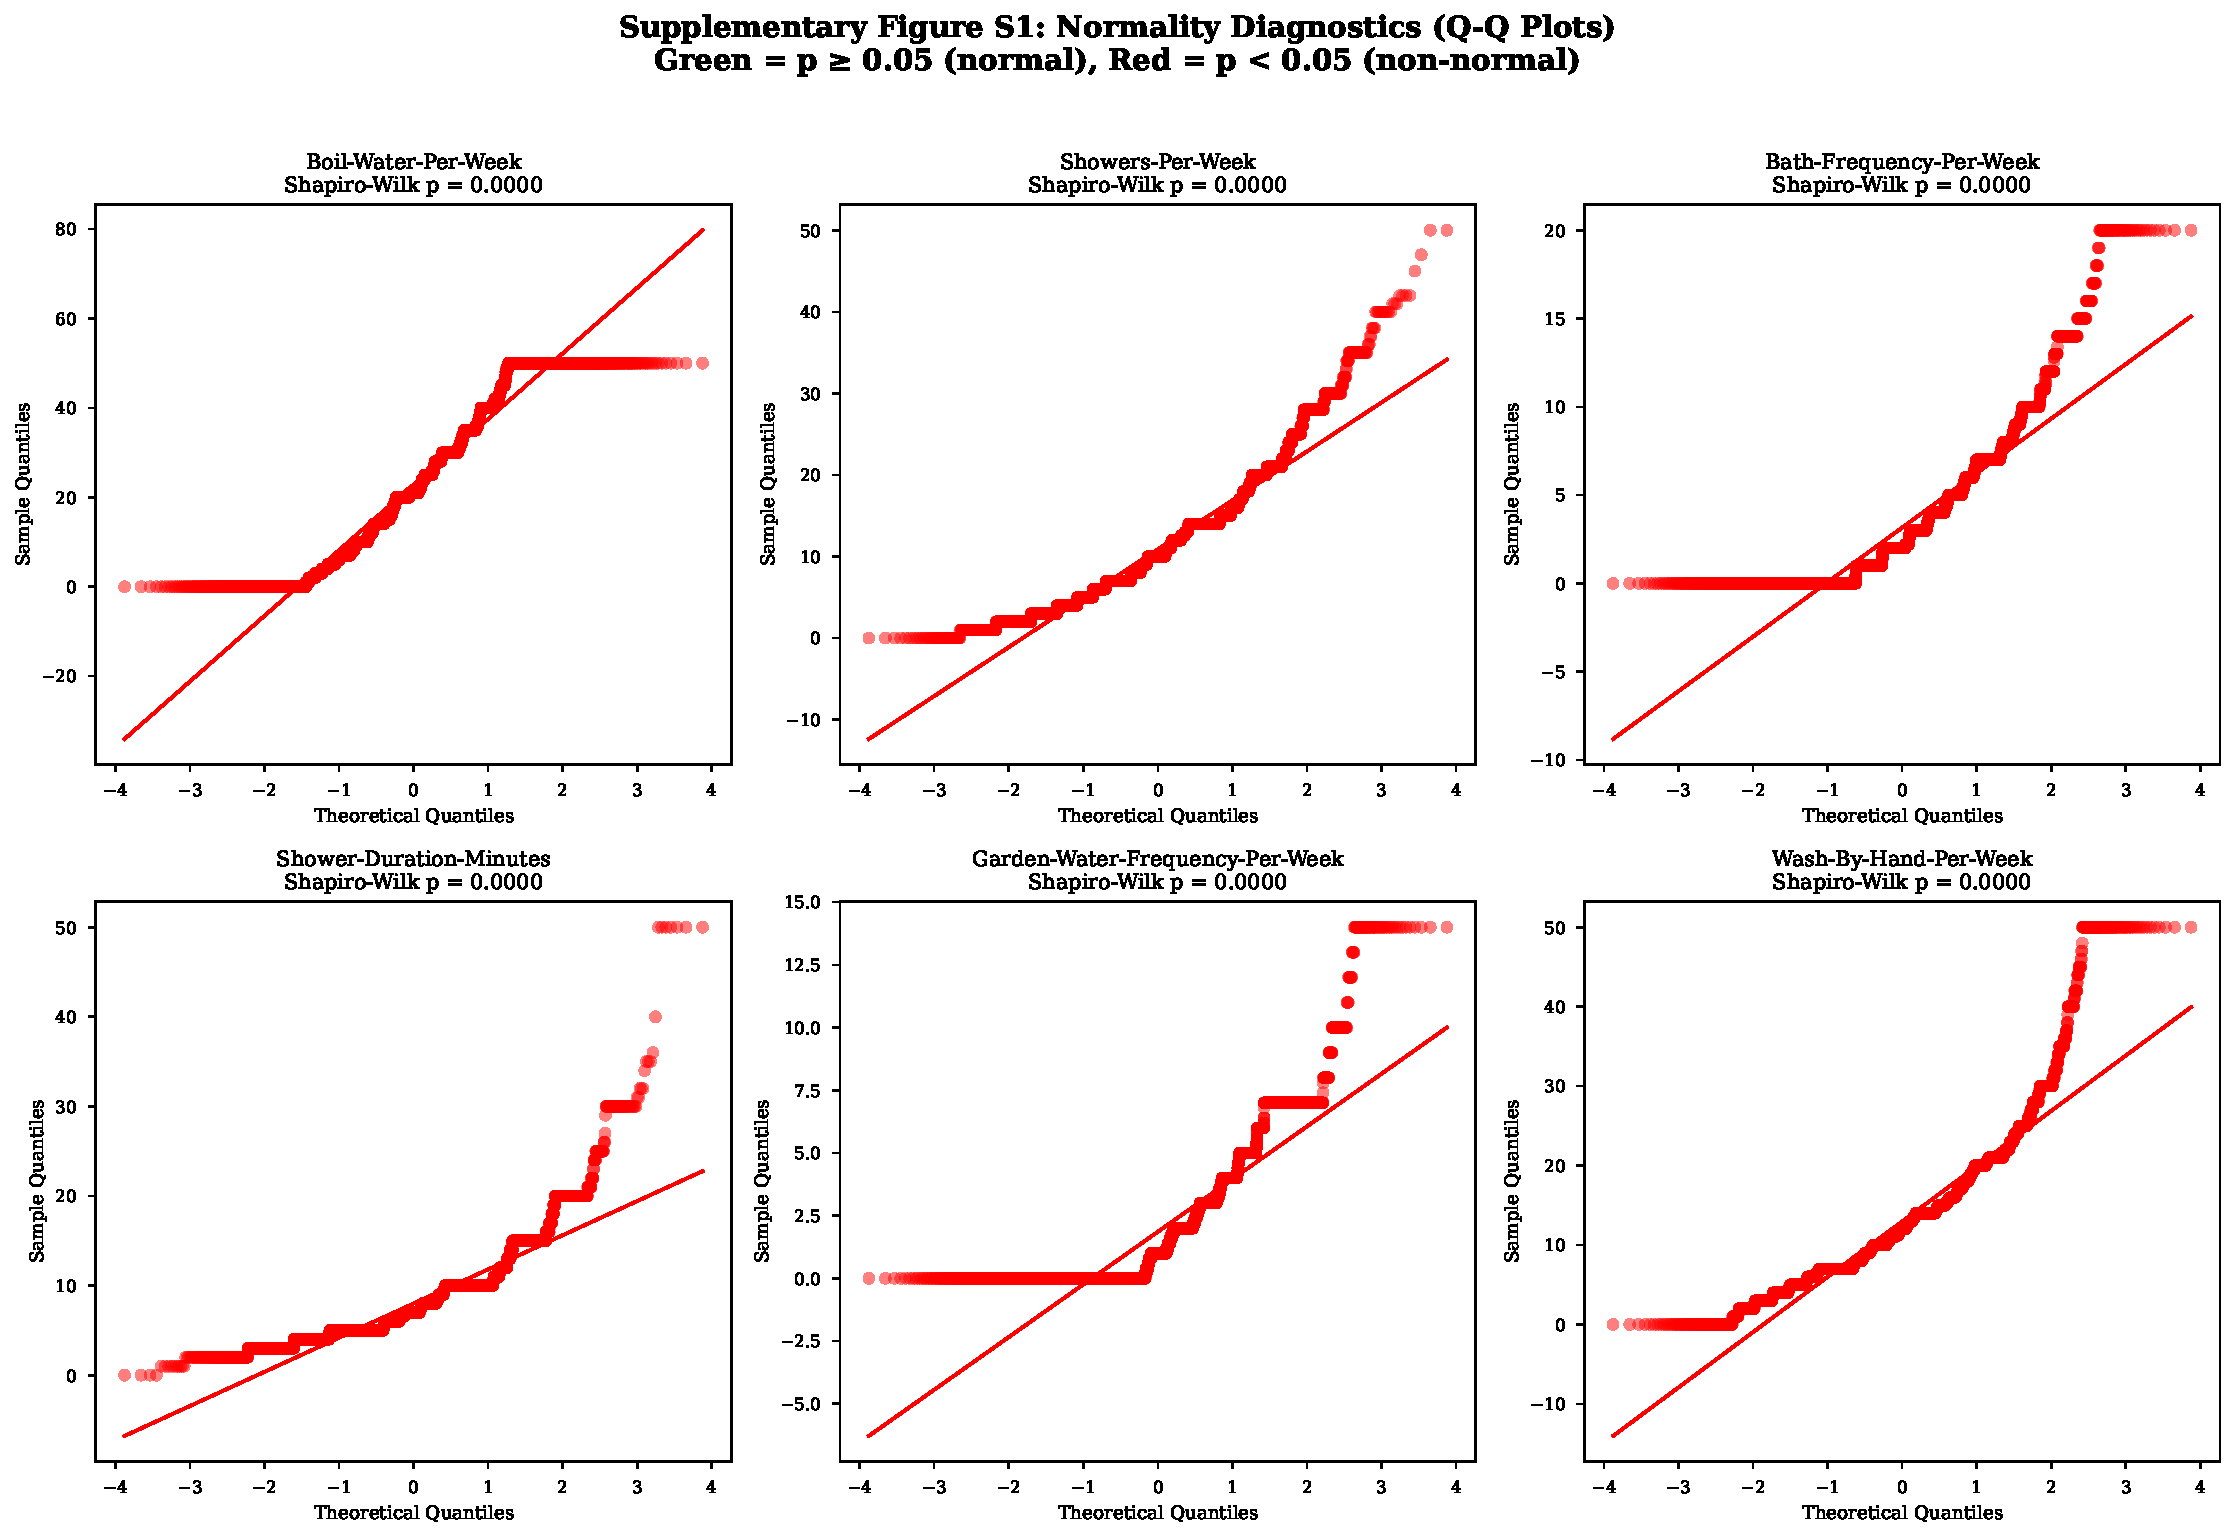
\includegraphics[width=\textwidth]{FigureS1_Normality_Diagnostics.pdf}
    \caption{Q-Q plots for top continuous variables showing departure from normality, justifying non-parametric validation approaches.}
\end{figure}

\subsection{Figure S2: Correlation Heatmap}
\begin{figure}[htbp]
    \centering
    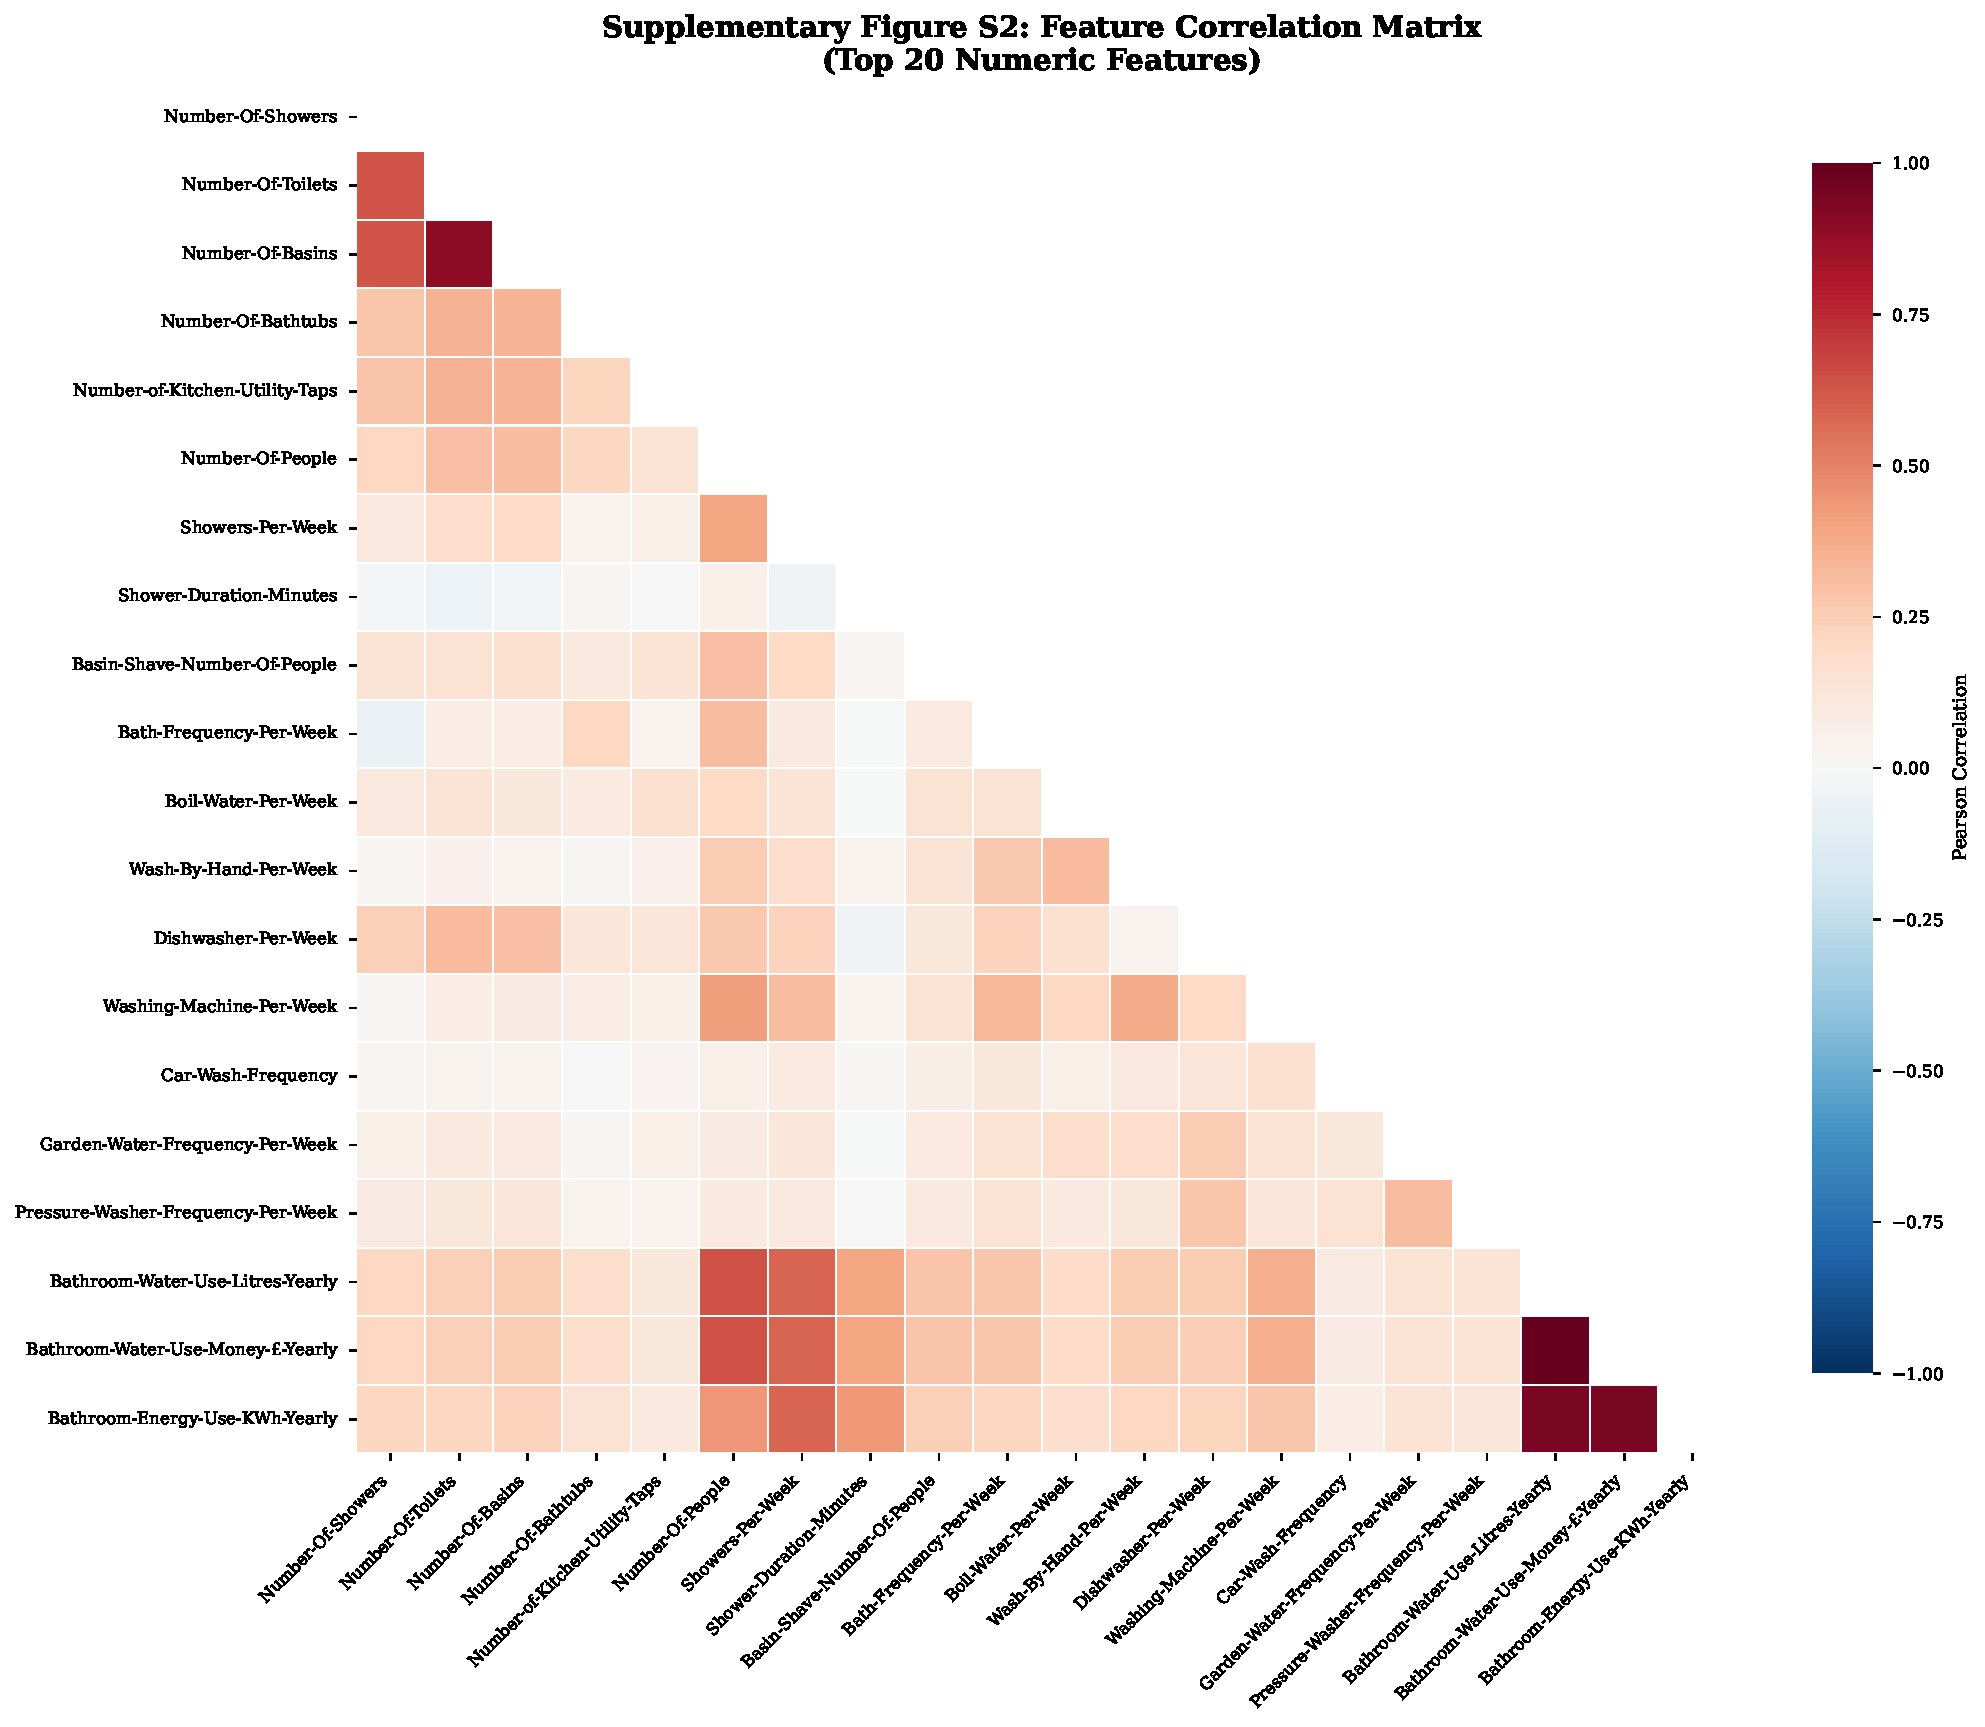
\includegraphics[width=0.9\textwidth]{FigureS2_Correlation_Heatmap.pdf}
    \caption{Correlation matrix for the 18 retained features after multicollinearity filtering. All pairwise correlations $|r| < 0.85$.}
\end{figure}

\newpage
\subsection{Figure S3: Cluster Distribution}
\begin{figure}[htbp]
    \centering
    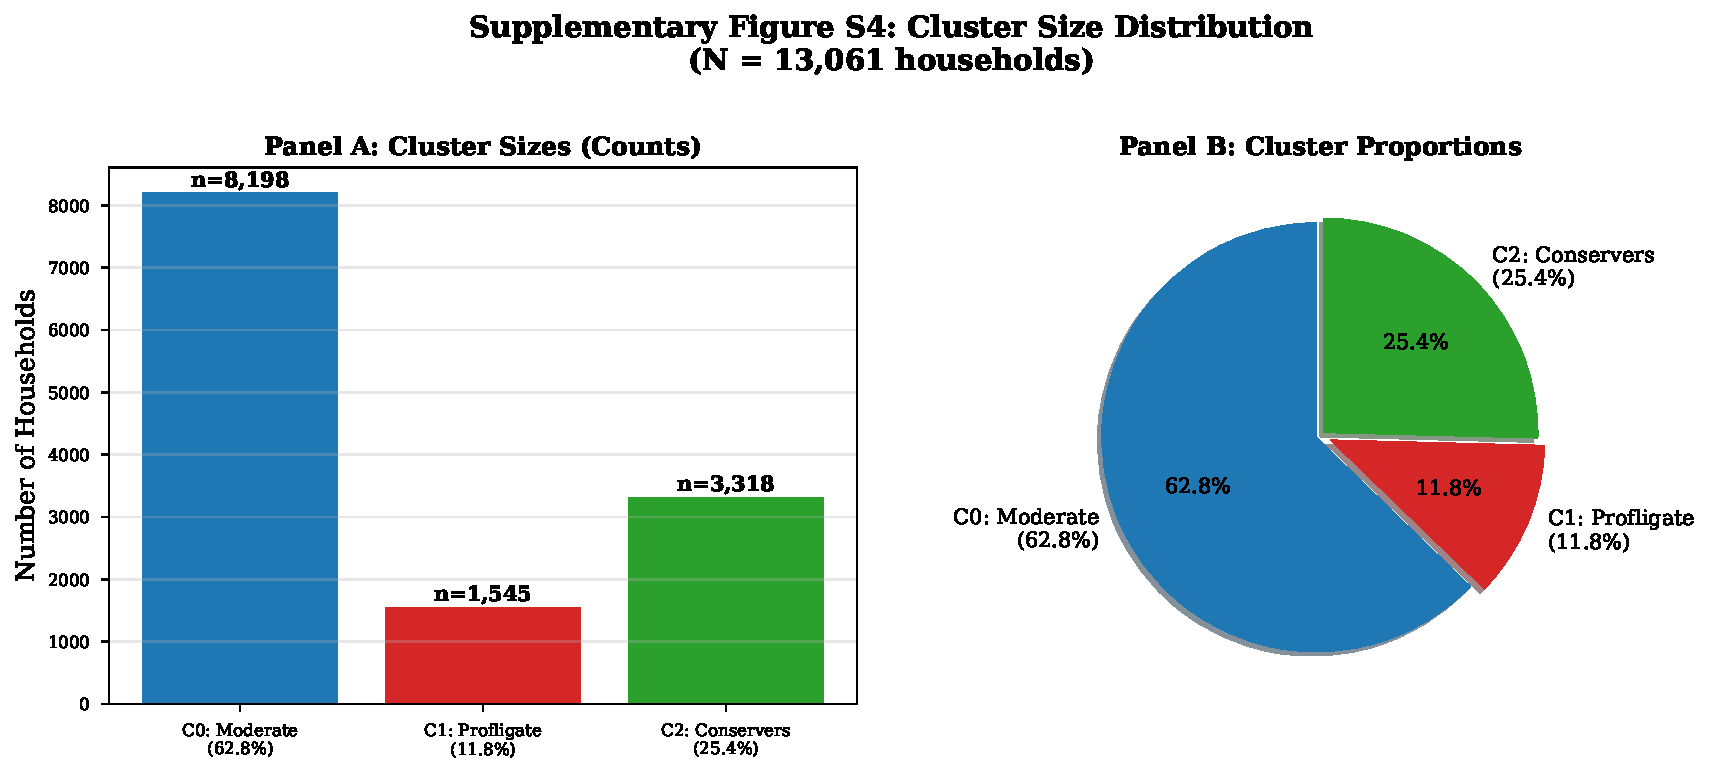
\includegraphics[width=0.8\textwidth]{FigureS4_Cluster_Distribution.pdf}
    \caption{Cluster size distribution showing Standard-Use (62.8\%), Low-Frequency (25.4\%), and High-Frequency (11.8\%) profiles.}
\end{figure}

\subsection{Figure S4: Feature Distributions}
\begin{figure}[htbp]
    \centering
    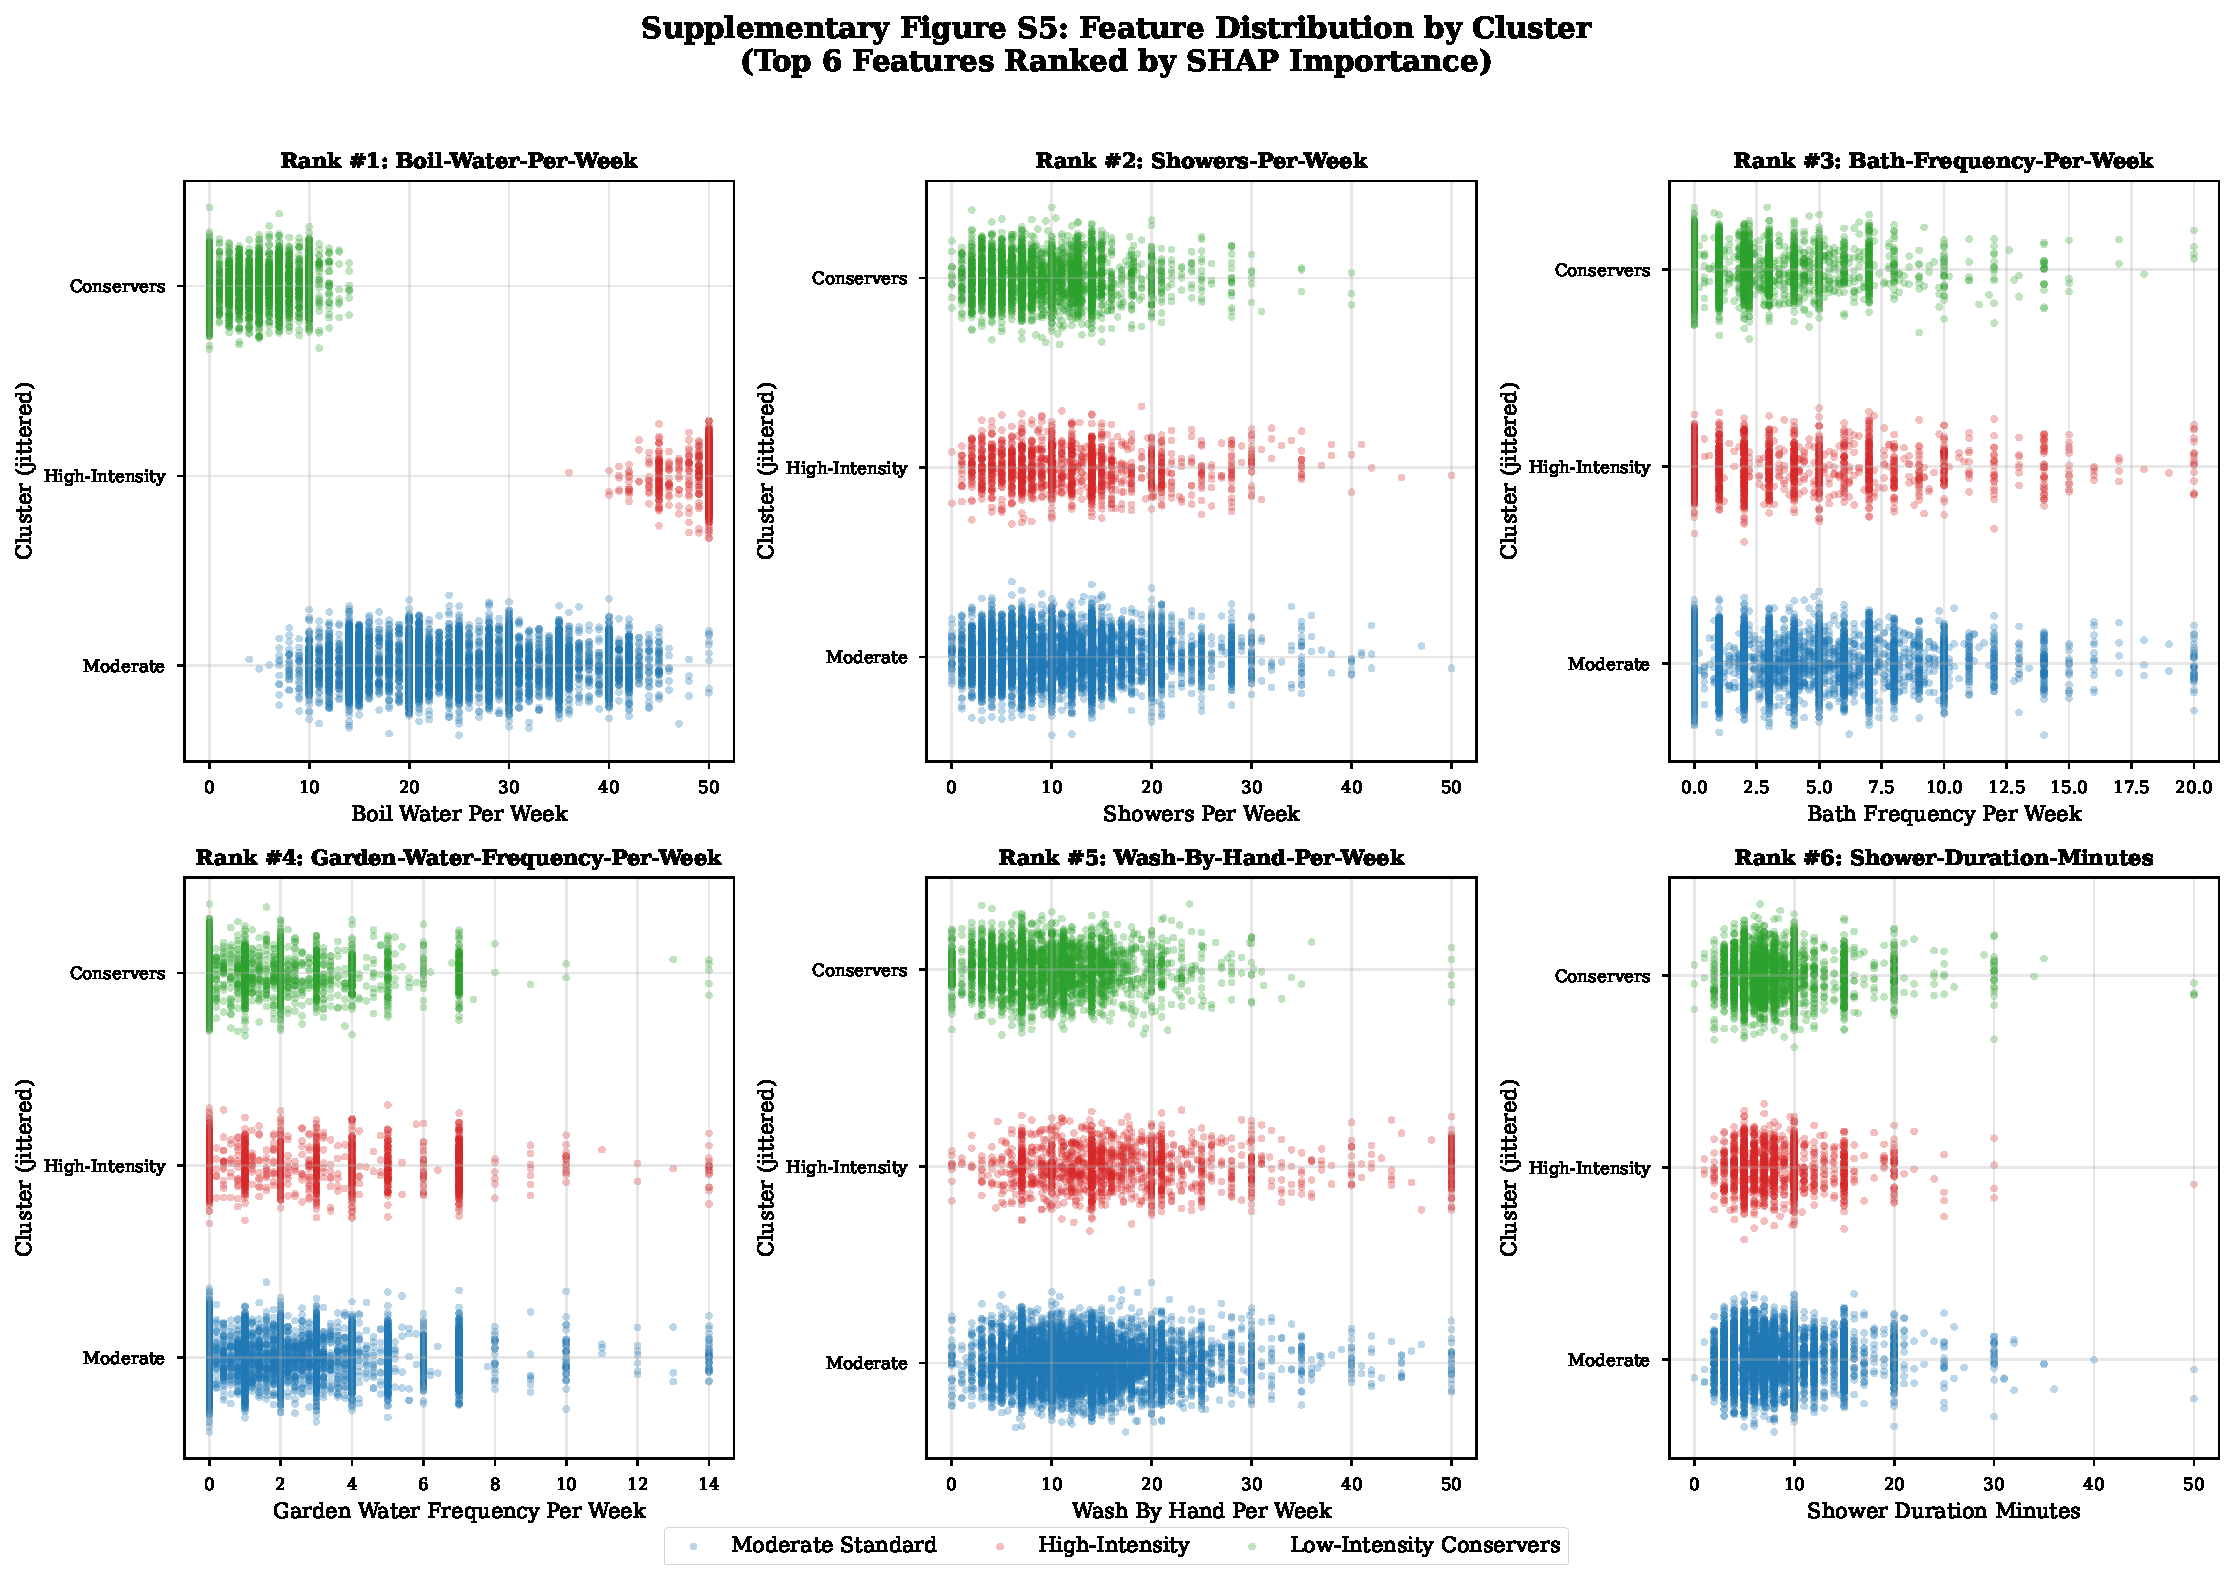
\includegraphics[width=\textwidth]{FigureS5_Feature_Distributions.pdf}
    \caption{Density plots for top behavioral features, separated by cluster assignment. Clear separation visible for boiling and bathing frequencies.}
\end{figure}

\newpage
\subsection{Figure S5: Interaction Effects}
\begin{figure}[htbp]
    \centering
    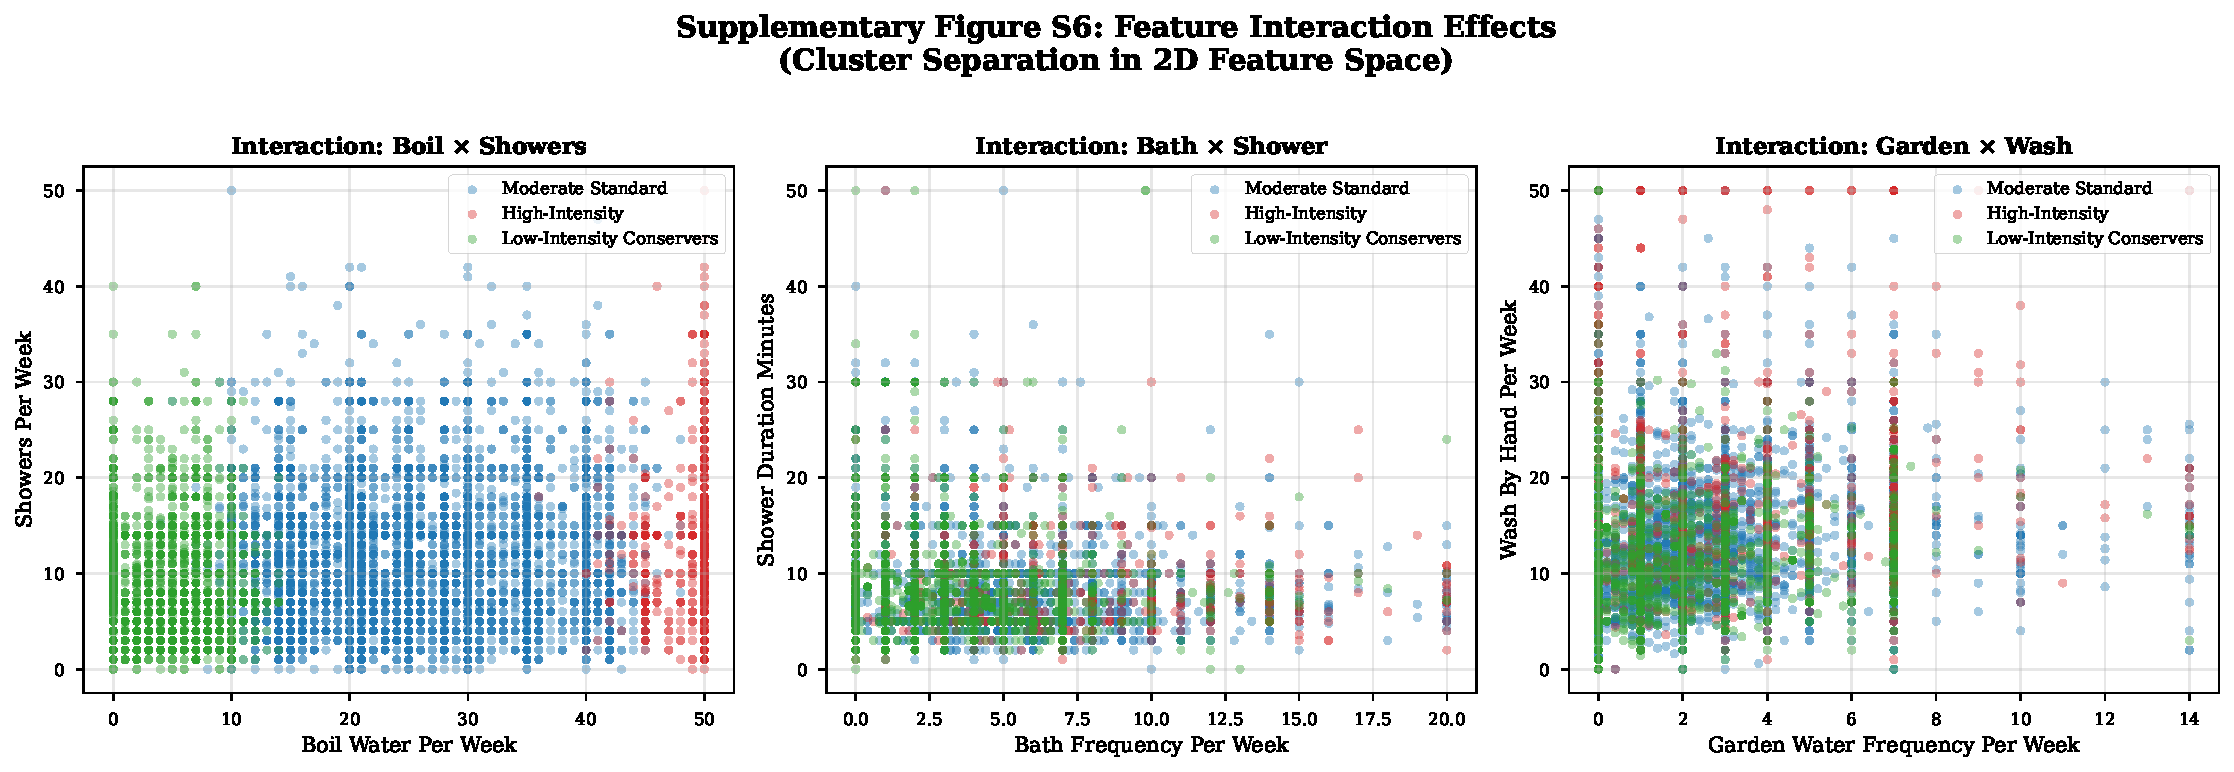
\includegraphics[width=\textwidth]{FigureS6_Interaction_Effects.pdf}
    \caption{SHAP interaction values between top feature pairs. Positive interactions (red) indicate synergistic effects on cluster classification.}
\end{figure}

\subsection{Figure S6: Box Plots}
\begin{figure}[htbp]
    \centering
    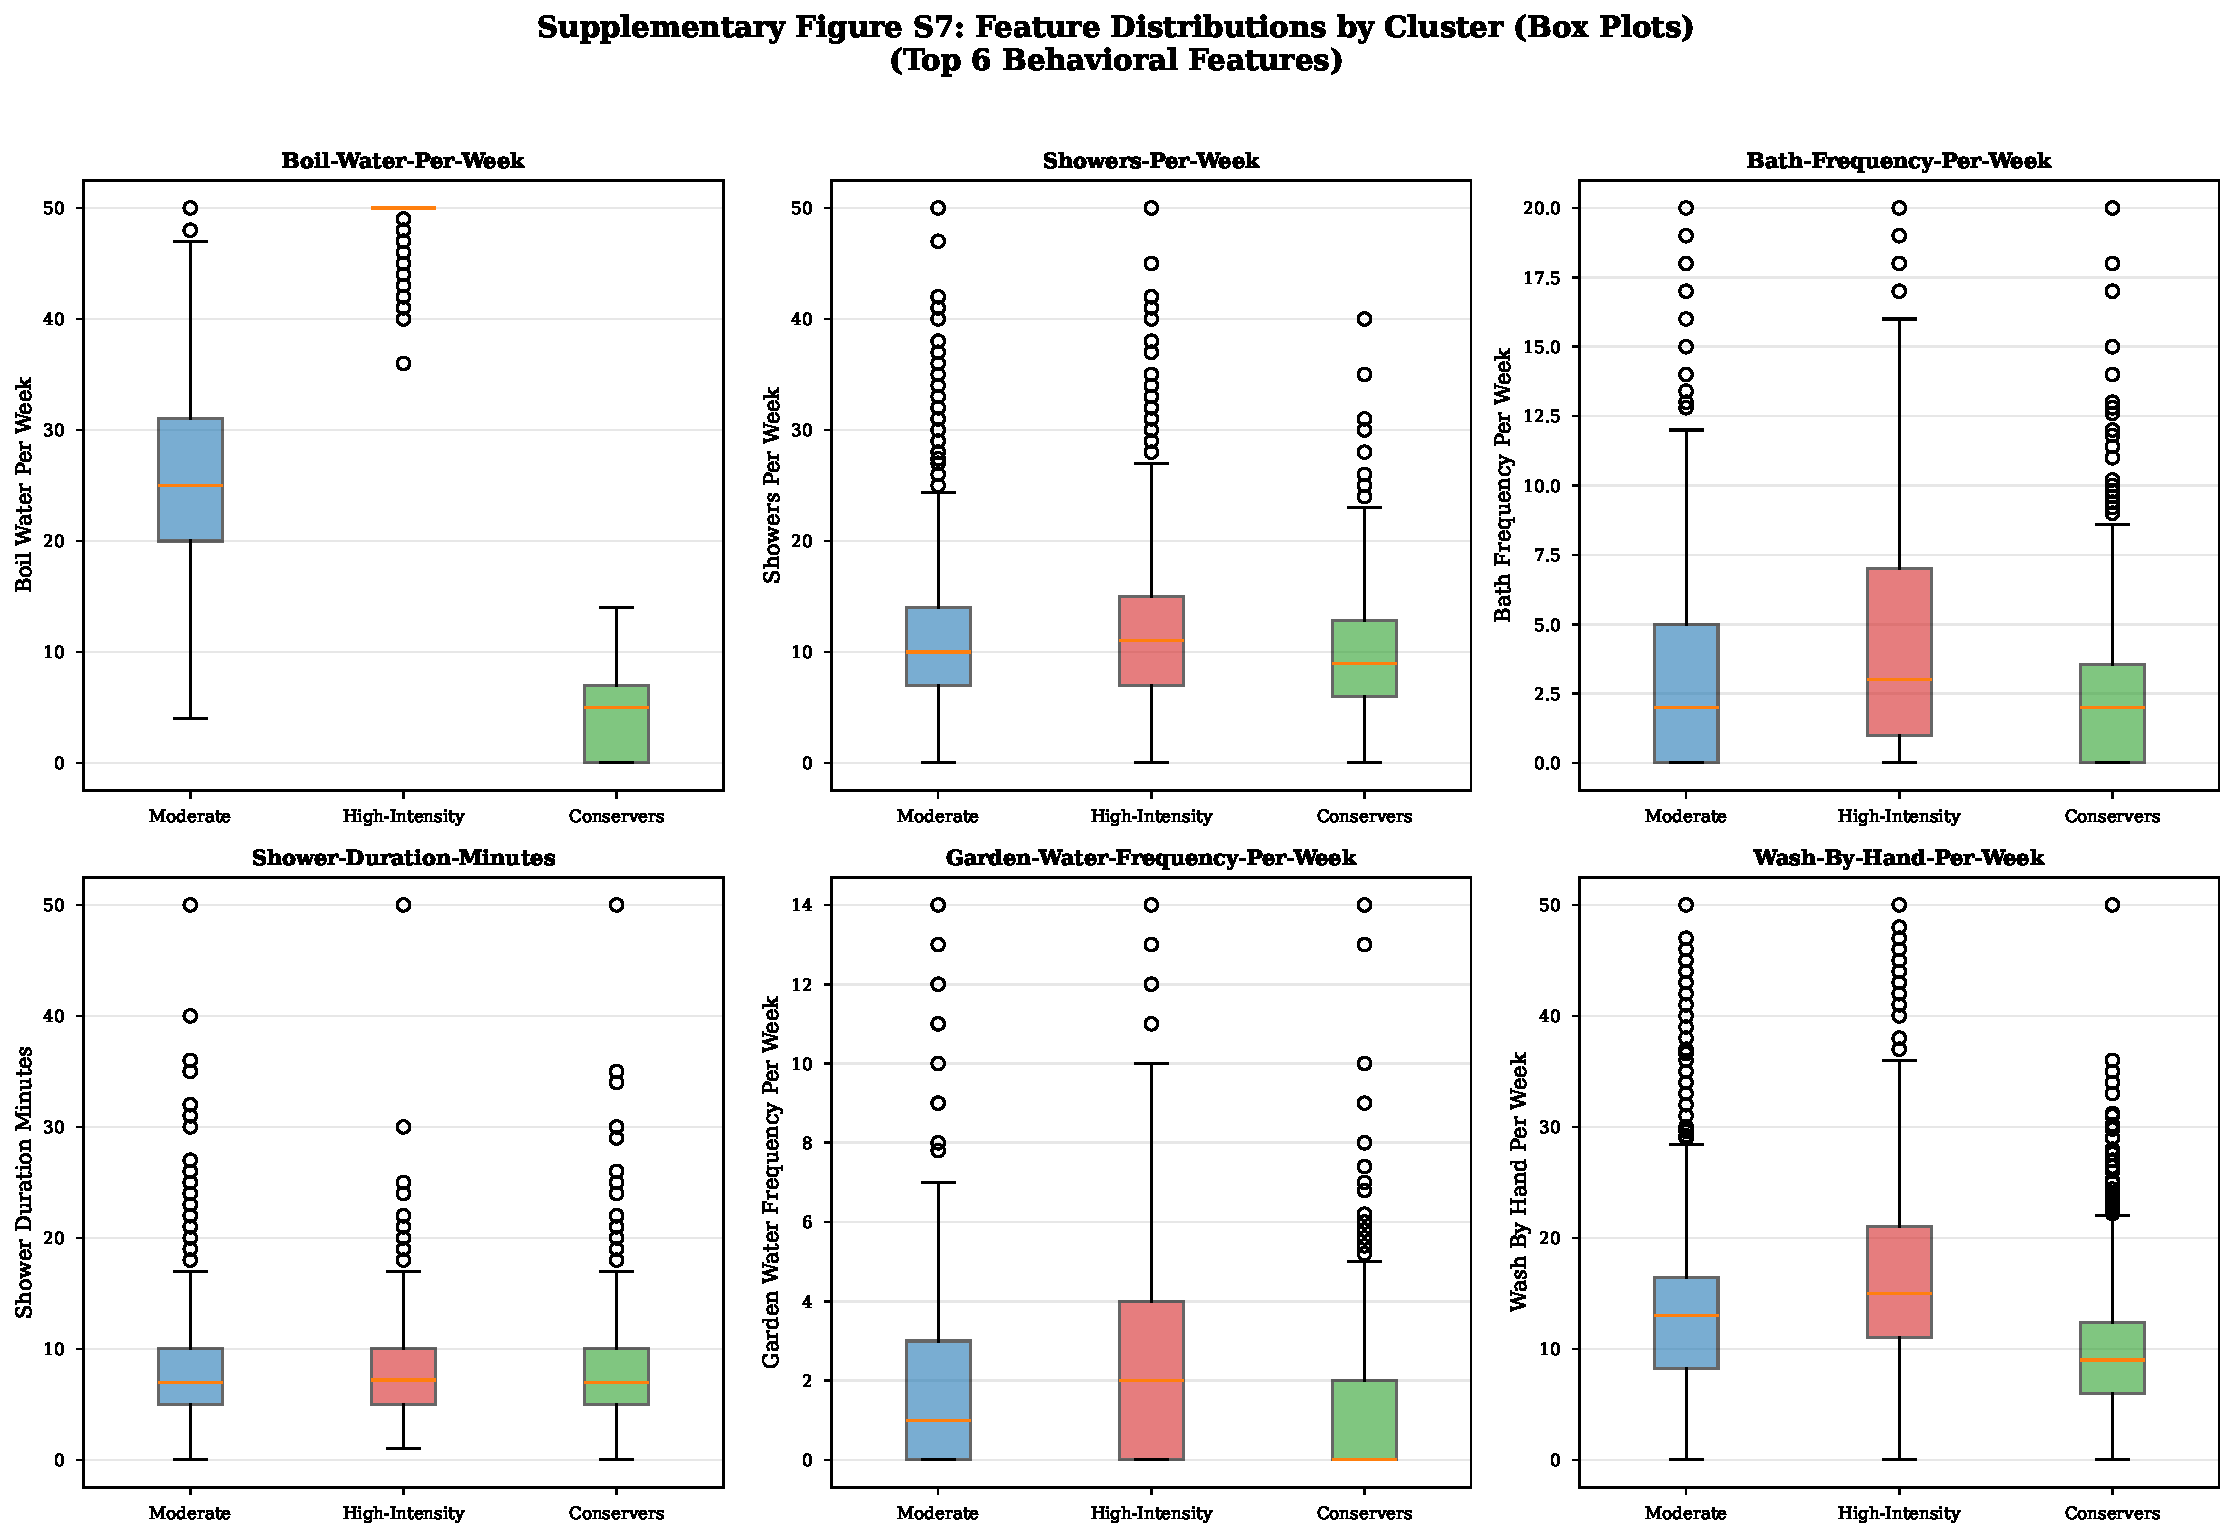
\includegraphics[width=\textwidth]{FigureS7_Boxplots.pdf}
    \caption{Box plots for key behavioral features across three clusters, illustrating distribution differences and outlier patterns.}
\end{figure}

% =============================================================================
% DATA AND CODE AVAILABILITY
% =============================================================================
\newpage
\section{Data and Code Availability}

\subsection{Data Availability}
The anonymized data supporting this study are available from Yorkshire Water upon reasonable request to the corresponding author, subject to data sharing agreements protecting customer privacy.

\subsection{Code Availability}
Python code for the analysis pipeline is available at: [GitHub repository URL to be added upon acceptance]

\textbf{Dependencies}:
\begin{itemize}
    \item Python 3.8+
    \item numpy, pandas, scikit-learn, scipy
    \item shap (for XAI analysis)
    \item matplotlib, seaborn (visualization)
\end{itemize}

Environment specification files (\texttt{requirements.txt}, \texttt{environment.yml}) are provided in the repository.

\end{document}
